\documentclass[10pt,twocolumn,letterpaper]{article}
\usepackage[review]{cvpr}
\usepackage{amsmath,amssymb,booktabs,graphicx,placeins}
\definecolor{cvprblue}{rgb}{0.21,0.49,0.74}
\usepackage[pagebackref,breaklinks,colorlinks,allcolors=cvprblue]{hyperref}
\def\confName{CVPR}
\def\confYear{2027}
\graphicspath{{figures/}}
\newcommand{\ReachPair}{79.4}
\newcommand{\ReachMark}{23.8}
\newcommand{\ReachImage}{64.2}
\newcommand{\AuditSave}{50.3}
\newcommand{\PCal}{67}
\newcommand{\UCal}{53}
\newcommand{\PTest}{105}
\newcommand{\UTest}{90}
\newcommand{\RoleTest}{69}
\newcommand{\PRank}{62}
\newcommand{\URank}{49}
\newcommand{\NHeads}{283}
\newcommand{\NHeadRows}{302}
\newcommand{\LowerHeads}{280}
\newcommand{\MoreHeads}{251}
\newcommand{\MedianDrop}{6}
\newcommand{\PastBand}{202}
\newcommand{\TopRemoved}{4}
\newcommand{\PairHitsP}{1}
\newcommand{\PairHitsU}{11}
\newcommand{\PairAlertsP}{0}
\newcommand{\PairAlertsU}{8}
\newcommand{\IwahitsP}{3}
\newcommand{\IwahitsU}{6}
\newcommand{\FirstHitsP}{4}
\newcommand{\FirstHitsU}{11}
\newcommand{\PairRank}{55}
\newcommand{\PairDrop}{7}
\newcommand{\PairControlHi}{4}
\newcommand{\PairCutoffP}{1.524}
\newcommand{\PairCutoffU}{0.630}
\newcommand{\PairChange}{17.1}
\newcommand{\PairChangeCI}{[7.5, 27.9]}
\newcommand{\PairRelativeP}{-4.0}
\newcommand{\PairRelativeU}{3.6}
\newcommand{\PairRelativePCI}{[$-7.0$, $-1.4$]}
\newcommand{\PairRelativeUCI}{[$-1.4$, 9.5]}
\newcommand{\ReferenceInteraction}{7.5}
\newcommand{\ReferenceInteractionCI}{[1.7, 14.4]}
\newcommand{\PairPrimary}{3.2}
\newcommand{\IpwPrimary}{7.1}
\newcommand{\PairRobustMedian}{0}
\newcommand{\OriginalLearned}{74}
\newcommand{\OriginalDescriptor}{47}


\title{Auditing Unmarked Nodules in the Patient Alert Tail\\
Supplementary Material}
\author{Anonymous}
\begin{document}
\maketitle

\section{Release, provenance and target geometry}

We indexed all 888 official LUNA16 series and verified each MetaImage header and raw volume against the corresponding release ZIP member's CRC and byte count. We validated Series Instance UID to TCIA patient links for the full inventory. Official subset counts are 89 each for subsets 0--7 and 88 each for 8--9. TCIA identity reveals one cross-subset repeat in subsets 2 and 6. We keep the earlier series. Two other scans in subset 2 have eight and three reading sessions, respectively, and are excluded. The remaining 885 series represent distinct patients (Tab.~\ref{tab:cohort}). Final test coverage is 274/276 targets, 42/42 observed omissions and 150/151 cap omissions. All official nodule annotations linked to at least one of the four released reader sessions under the geometry check on this cohort.

\begin{table}[t]
\centering\small
\caption{\textbf{Patient splits under the original C/D reference.} Neg. counts reference-negative patients. Obs. omit. counts first-reader omissions.}
\label{tab:cohort}
\begin{tabular}{lrrrr}
\toprule
Split & Patients & Neg. & Targets & Obs. omit. \\
\midrule
Train & 445 & 152 & 541 & 92 \\
Cal & 175 & 67 & 215 & 34 \\
Test & 265 & 105 & 276 & 42 \\
\bottomrule
\end{tabular}

\end{table}

The V2 false-positive reduction roster extends the original merged candidate set with outputs from ETROCAD and M5LCADThreshold0.3 \cite{setio2017,luna16v2}. Components were developed using multiple sources including LIDC-IDRI and, for LargeCAD, the LUNA16 source dataset. Some full CAD submissions used LUNA16 cross-validation. Exact per-series development exposure of each V2 coordinate is unavailable. We discard the supplied class column and use identical coordinates in all arms. The upstream proposal set conditions both coverage and the negative tail. Official FROC uses a different target definition and ignores some non-target marks. Our counts use the operational reference in the main paper.

For each released contour mark we use positive-inclusion regions, convert pixel coordinates and the slice's physical position to millimeters and take the bounding-box midpoint. The mark size is the largest axis-aligned in-plane extent across slices. For two mark sets, we use one-to-one minimum normalized-distance assignment subject to a distance at most $\max(3\,\mathrm{mm},(d_1+d_2)/4)$, prioritizing match count. The mean center and diameter of each linked C/D pair define a target. A proposal links to the closest target within one normalized radius where the scale is $\max(3\,\mathrm{mm},d/2)$. A target's omission status uses an independent one-to-one link with the first weak read. The signed spacing and origin in the MetaImage header determine the correspondence. The original roles and matching rules are shared across revisions. No missing weak streams occur after requiring four sessions in this benchmark. The discriminative auxiliary still encodes availability explicitly.

An unmatched proposal is \emph{disputed} if it links to an isolated contour marked by only one reference role. The released final LIDC reader records follow an unblinded phase \cite{armato2011}. An isolated contour signals disagreement in the operational reference. No independent diagnostic adjudication of those candidates was collected. A sibling patient-level inventory review found no previously unexposed official positive nodules in subsets 6--9 under its definition of exposure. The present weights and heads were developed without revision scores from subsets 2 and 6--9. We describe the evaluation as retrospective and locked.

\section{Representation and optimization}

\paragraph{Handcrafted features.}
Around each candidate we interpolate a $13^3$ grid at 1.5\,mm spacing, clip to $[-1100,400]$ HU and scale by 1000. Four radial shells supply mean, standard deviation and the fraction above $-300$ HU. Four scales of Gaussian/Hessian features supply a smoothed intensity, three eigenvalues and a curvature roundness ratio \cite{li2003}. This yields 32 descriptors.

\paragraph{Patch encoder.}
The selected 3D network receives a $24^3$ crop on a physical 1\,mm grid. We clip to $[-1050,400]$ HU, quantize to 8-bit storage and scale to $[-1,1]$. Two convolution blocks at each width 16, 32 and 48 use $3^3$ kernels, batch normalization and SiLU. Pooling by two follows the first two widths. We concatenate global average pooling and a central $4^3$ pooled region, then apply a 32-channel linear map, layer normalization and SiLU. A weak-mark linear readout trains the embedding. At export we average the embedding of the original patch and its separate flips in the two in-plane axes.

The encoder fit uses 267 unique patients in subsets 0, 1 and 3 and reads only the arm's first-role marks. No pretrained weights or reference labels enter this fit. Each epoch uses 72 minibatches of 192 proposals, with 32 marked and 160 unmarked samples. After epochs 4, 10 and 16 we refresh the hard pool from the highest 2.5\% of unmarked scores. Forty-eight unmarked draws per batch use that pool, and the rest use the full unmarked set. We use reflections, axis swaps, affine HU jitter, smoothed binary labels 0.01/0.99 and AdamW with a cosine schedule from $1.5{\times}10^{-3}$ to $1.5{\times}10^{-4}$. The epoch-16 checkpoints are frozen after a 24-epoch development schedule. The fitted head receives the standardized 32-dimensional embedding. The two arms have separate weights because the cap drops first-role marks during encoder fit.

We first tested a multiscale 2.5D model with twelve orthogonal slices at two fields of view, across three saved epochs and two ridge values. It improved candidate separation but missed the all-target localization gate. The bounded repair compared rank-weighted heads and one 3D fit per arm. The frozen gate required a ten-point improvement in all-target recall and an improvement in within-scan target separation, with negative alerts within five points. The unweighted 3D model passed. The development ledger retains the two ridge values, all diagnostic cutoffs and both patch architectures.

\paragraph{Common head.}
We standardize features on fit candidates and use a linear logistic logit with coefficient ridge $10^{-4}$ and intercept penalty $10^{-6}$. Optimizing an augmented loss uses its exact linear label moment. Loss curvature with respect to the score is independent of the target, including for signed values. Positive ridge bounds the optimization. IPW uses logistic loss on revealed examples weighted by $1/\pi_i$ and normalized by the sum of these weights. The nnPU baseline treats A marks as positives and uses the Horvitz--Thompson prior estimate, clipped to a positive interior value. We optimize its convex nonnegative risk. The EM image and reader heads use the working two-reader likelihood. Starting from the IPW image head, we alternate 16 updates with audited labels clamped. The positive-reference mark probability has a logistic head with ridge 0.02 for each reader. Its negative-reference rate is a smoothed constant.

\section{Sampling and cross-fitting details}

\paragraph{Weak evidence for allocation.}
Within each of three training patient folds, predict the union of the weak marks using a logistic image model fit on the other folds. Let $p_i$ be that prediction and $m_i$ the number of observed marks. Our proxy $u_i$ is $0.35p_i$ for $m_i=0$, $0.55+0.35p_i$ for $m_i=1$, and $0.92+0.06p_i$ for $m_i=2$. These fixed coefficients downweight the uncertainty of clear agreements and elevate informative disagreements. They define a design heuristic. The use of both a rank within a scan and a common absolute cutoff retains candidates that can affect an extreme scan score even when scan-level intensity distributions differ. The design is frozen before any reference reveal. For $\pi_i$ away from a box constraint, differentiating the surrogate objective plus the budget multiplier gives $\pi_i=c\,h_i\sqrt{v_i}$. The same argument gives the clipped solution with the stated floors, cap and truncated $h_i$.

\paragraph{Conditional loss.}
Let $\mathcal F_{-f}$ contain the pre-audit data and all training audit uniforms outside patient fold $f$. Conditional on $\mathcal F_{-f}$ and the finite-pool $Y$, the independent uniforms in fold $f$ leave $\Pr(R_i=1)=\pi_i$ and $q_i$ is fixed. For any fixed $g$ and pre-audit weights $a_i$,
\[
 \mathbb E_R\!\left[\frac{\sum_i a_i\ell(z_i,g_i)}{\sum_i a_i}\right]
 =\frac{\sum_i a_i\ell(Y_i,g_i)}{\sum_i a_i}.
\]
This includes the unit-weight and tail-weighted objectives. The weighted estimand gives extra mass to candidates ranked near the frozen tail. It is independent of the choice of inclusion probabilities.

\paragraph{Power.}
Write $\bar X_i$ for the standardized design vector with intercept. We select $\lambda$ by minimizing an estimate of
$\sum_i(1-\pi_i)(Y_i-\lambda q_i)^2\|\bar X_i\|^2/\pi_i$.
For each outer fold, we predict the discriminative auxiliary on the other folds using an inner split and estimate this criterion using audited labels and an additional factor of $1/\pi_i$. The quadratic minimizer is clipped to $[0,1]$. The held fold uses the scaled prediction from a full auxiliary fit on the other folds. This is a fixed-fold scalar variance-tuning comparator inspired by prediction-powered training \cite{ppssl2025}. It uses the same labels and head as the untuned discriminative fit.

\paragraph{Audit reach and variability.}
For reference target $j$ with eligible proposal indices $\mathcal I_j$, its expected audit exposure is $1-\prod_{i\in\mathcal I_j}(1-\pi_i)$. Sum over targets or the omission subgroup. The empty product is one. This calculation uses the retrospective full fit reference only for evaluation. It estimates reach in the training pool. The gradient ledger records squared residuals, audited signed residual extremes and the diagonal contributions to design variance of the label moment. Conditional on a fold's auxiliary fit, its residual terms are independent under the design. The reported sum of conditional diagonal terms does not include between-fold covariances from fitting auxiliaries on shared labels. We also record realized gradient errors across draws and the evaluation-only Brier error of auxiliaries by weak-mark pattern.

\begin{center}
\small
\captionsetup{hypcap=false}
\captionof{table}{\textbf{Evaluation-only auxiliary error.} Mean squared residual ($\times 10^3$) by test proposal mark pattern at the learned, mark-stratified anchor. Ref. is the observed candidate prevalence.}
\label{tab:aux}
\begin{tabular}{lrrrrr}
\toprule
Marks & $N$ & Ref.\% & Image & Disc. & EM \\
\midrule
00 & 224,631 & 0.016 & 0.36 & 0.16 & 0.17 \\
01 & 203 & 27.586 & 200.85 & 190.49 & 550.87 \\
10 & 169 & 14.793 & 128.08 & 116.97 & 573.15 \\
11 & 472 & 70.763 & 253.43 & 197.39 & 292.23 \\
\bottomrule
\end{tabular}

\end{center}

\section{Prespecified comparisons and operating points}

The final confirmatory status is locked retrospective re-evaluation. The primary half-budget contrast was selected using subsets 4 and 5 for calibration and evaluation, respectively. In development the selected method's six-draw omission recall was 23.3\%, versus 18.3\% for base-budget mark-stratified IPW at 8.6\% mean alerts each. nnPU with an audited class prior had 28.3\% omission recall across its three development draws and was kept as a separate comparator. For a gain claim the locked rule required +10 pp versus first read and +5 pp versus the strongest simple audited comparator, positive paired lower limits, and positive effects against the audited comparator in at least four of six draws. The selected efficiency route required at least a 25\% candidate saving and lower paired limits above or equal to $-5$ pp for both recall measures. Both routes required at most 13\% realized negative alerts, at most +3 pp relative to the audited comparator and at most +0.20 FP/scan. We report the selected route regardless of outcome.

We resample test patients in pairs 4,000 times with fixed weights across the six matched audit seeds for the averaged effect. The anchor interval conditions on one draw and the pooled calibration set. For the separate calibration sensitivity we jointly resample the 67 negative patients 300 times with replacement, then recompute each strict cutoff. The audit seeds and calibration resamples use the same test cases. The two-stage matched-alert check uses negative patients from subset 2 to obtain a grid of thresholds and subset 6 to select the highest attained alert rate at or below 10\%, preferring the higher cutoff when tied. This check is separate from the pooled conformal guarantee.


\begin{table*}[t]
\centering\small
\caption{\textbf{Observed-read supervision factorial at the anchor.} Cells report detections among 42 observed omissions and 276 total targets, followed by alerts among 105 C/D-negative test patients. Audited methods share the base mark-stratified draw.}
\label{tab:observed}
\begin{tabular}{lcc}
\toprule
Supervision & Descriptors & 3D features \\
\midrule
First read & 2 / 39 / 12 & 4 / 81 / 2 \\
Second read & 2 / 37 / 12 & 1 / 76 / 3 \\
nnPU & 2 / 40 / 12 & 3 / 59 / 2 \\
Audit-only IPW & 2 / 57 / 14 & 3 / 70 / 5 \\
Paired EM & 2 / 44 / 12 & 3 / 76 / 3 \\
Image augmentation & 2 / 55 / 12 & 4 / 69 / 5 \\
Discriminative augmentation & 2 / 47 / 11 & 1 / 68 / 4 \\
EM augmentation & 2 / 48 / 10 & 2 / 71 / 6 \\
Power-tuned augmentation & 2 / 48 / 11 & 1 / 69 / 4 \\
Full reference & 2 / 47 / 12 & 1 / 74 / 2 \\
\bottomrule
\end{tabular}

\end{table*}

\begin{figure*}[t]
\centering
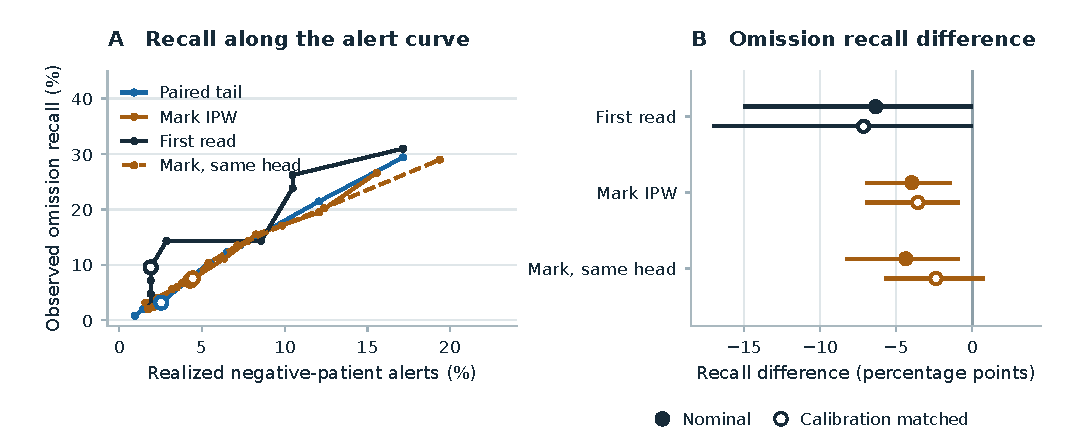
\includegraphics[width=\textwidth]{locked_performance}
\caption{\textbf{Locked operating points and paired effects.} (A) Every point uses a calibration-derived cutoff, and open markers denote nominal $\alpha=0.10$. (B) Paired-tail omission recall minus each comparator, with patient-clustered intervals. Open markers use the calibration-only matched-alert check.}
\label{fig:locked}
\end{figure*}

\begin{table}[t]
\centering\small
\setlength{\tabcolsep}{3.5pt}
\caption{\textbf{Bookmark cap factorial.} Each cell reports anchor detections among 151 imposed omissions, all 276 targets, and alerts among 105 reference-negative patients. The cap arm's encoder trains on the cap's first-read labels.}
\label{tab:cap}
\begin{tabular}{lcc}
\toprule
Supervision & Descriptors & 3D features \\
\midrule
First read & 31 / 61 / 16 & 25 / 81 / 4 \\
Second read & 22 / 37 / 12 & 30 / 88 / 5 \\
nnPU & 32 / 62 / 16 & 25 / 81 / 4 \\
Audit-only IPW & 29 / 57 / 15 & 32 / 96 / 4 \\
Paired EM & 24 / 43 / 11 & 33 / 98 / 4 \\
Image augmentation & 28 / 55 / 13 & 33 / 97 / 4 \\
Discriminative augmentation & 26 / 51 / 12 & 34 / 96 / 4 \\
EM augmentation & 24 / 46 / 10 & 37 / 98 / 5 \\
Power-tuned augmentation & 26 / 51 / 13 & 34 / 96 / 4 \\
Full reference & 26 / 47 / 12 & 38 / 104 / 7 \\
\bottomrule
\end{tabular}

\end{table}

\begin{table*}[!t]
\centering\small
\caption{\textbf{Paired effects at the locked and calibration-matched operating points.} Differences are percentage points except FP/scan. Patient intervals use the matched-draw mean.}
\label{tab:contrasts}
\begin{tabular}{llrrrr}
\toprule
Contrast & Threshold & $\Delta$ Omit. [95\%] & $\Delta$ All & $\Delta$ Alert & $\Delta$ FP/scan \\
\midrule
Selected vs. base IPW & Nominal & -4.0 [-7.0, -1.4] & +3.02 & -1.75 & -0.01 \\
Selected vs. first read & Nominal & -6.3 [-15.1, +0.0] & -6.22 & +0.63 & -0.06 \\
Selected vs. nnPU & Nominal & -4.0 [-11.5, +1.1] & +0.48 & +0.63 & -0.05 \\
Paired vs. mark (same fit, half) & Nominal & -4.4 [-8.3, -0.8] & -1.33 & -1.90 & -0.01 \\
Paired vs. image tail (same fit, half) & Nominal & -1.6 [-3.7, +0.0] & -0.12 & +0.16 & -0.02 \\
Disc. vs. image aug. (mark) & Nominal & -1.2 [-3.0, +0.5] & +0.66 & -0.95 & -0.03 \\
EM vs. disc. aug. (mark) & Nominal & +0.0 [-2.5, +2.1] & -0.36 & +0.32 & -0.00 \\
EM aug. vs. IPW (mark) & Nominal & -0.8 [-5.7, +3.9] & -5.31 & -0.95 & -0.10 \\
EM aug. vs. first read (mark) & Nominal & -4.0 [-13.8, +4.3] & -11.96 & +2.22 & -0.14 \\
EM aug. vs. image aug. (mark) & Nominal & -2.4 [-7.3, +2.3] & -5.68 & -1.27 & -0.10 \\
Power vs. disc. aug. (mark) & Nominal & +0.0 [+0.0, +0.0] & -0.91 & +0.00 & +0.01 \\
Tail-weighted vs. unit-weight disc. & Nominal & -0.4 [-1.9, +1.0] & +2.90 & +0.16 & -0.01 \\
3D vs. descriptors (full ref.) & Nominal & -2.4 [-11.4, +5.6] & +9.78 & -9.52 & +0.02 \\
3D vs. descriptors (first) & Nominal & +4.8 [+0.0, +12.5] & +15.22 & -9.52 & +0.07 \\
Selected vs. base IPW & Matched & -3.6 [-7.0, -0.9] & +0.30 & -1.11 & -0.01 \\
Selected vs. first read & Matched & -7.1 [-17.1, +0.0] & -13.35 & -0.16 & -0.12 \\
Selected vs. nnPU & Matched & -4.8 [-12.7, +0.5] & -5.80 & -0.16 & -0.10 \\
Paired vs. mark (same fit, half) & Matched & -2.4 [-5.7, +0.8] & -2.42 & -1.59 & -0.02 \\
\bottomrule
\end{tabular}

\end{table*}

\begin{table*}[!t]
\centering\small
\caption{\textbf{Audit allocation and audit workload.} Mean across matched repeats. Each row shares candidate reveals across eligible heads. Lesions counts distinct audited reference targets. Omit.\ denotes distinct audited observed omissions. The expected reach uses all fitting targets and their audit probabilities.}
\label{tab:costs}
\begin{tabular}{lrrrrrrrr}
\toprule
Policy & Budget & Candidates & Pos. cand. & Lesions & Omit. & Patients & Exp. omit. & Exp. dbl. unmarked \\
\midrule
Mark stratified & 0.5 & 3,942 & 84 & 75.7 & 14.0 & 443.5 & 13.0 & 0.4 \\
Mark stratified & 1 & 7,933 & 169 & 142.0 & 24.2 & 445.0 & 23.8 & 0.9 \\
Uniform & 0.5 & 3,938 & 9 & 8.5 & 1.0 & 443.3 & 1.4 & 0.5 \\
Uniform & 1 & 7,938 & 15 & 15.0 & 2.3 & 444.8 & 2.7 & 0.9 \\
Image tail & 0.5 & 3,939 & 571 & 431.3 & 65.5 & 445.0 & 64.2 & 22.6 \\
Image tail & 1 & 7,892 & 665 & 490.0 & 80.8 & 445.0 & 79.7 & 29.1 \\
Paired tail & 0.5 & 3,940 & 652 & 482.7 & 79.2 & 444.8 & 79.4 & 27.4 \\
Paired tail & 1 & 7,898 & 689 & 502.2 & 86.2 & 445.0 & 84.6 & 30.2 \\
\bottomrule
\end{tabular}

\end{table*}

\paragraph{Sparse strata and gradient variance.}
At the anchor draw, mark stratification audits none of the 61 reference-positive training candidates without any weak mark, and every audited label in this stratum is multiplied by $1/\pi=50$. With the image-only auxiliary, the realized signed residual correction in this stratum ranges from $-36.51$ to approximately zero, compared with $-0.36$ to approximately zero for the discriminative auxiliary. Using the weak marks thus reduces the auxiliary error in this stratum (Tab.~\ref{tab:aux}), although the deployed head remains limited by both ranking and calibration.

For candidates without any weak mark, the diagonal design variance of the discriminative moment is $5.67{\times}10^{-6}$ under base-budget mark allocation and $1.44{\times}10^{-6}$ under half-budget paired-tail allocation. Weighting the gradient by the frozen leverage $h_i$ gives $3.22{\times}10^{-6}$ and $4.10{\times}10^{-9}$, respectively; this diagnostic is computed on the same tail that guided the allocation. Candidates away from the tail can still receive large inverse probabilities: under half-budget paired-tail allocation, the scaled residuals in this stratum range from $-0.91$ to $8.45$. The power-tuned multipliers at the anchor draw are 0.67, 0.90 and 0.38, and over the six base-budget mark draws the power-tuned and untuned discriminative heads yield identical omission and alert counts at the primary threshold. All-target recall, in contrast, is sensitive to the head objective across the development grid of ridge penalties and loss weights.

\paragraph{Controlled bookmark cap.}
In this setting, the first reader retains only its largest mark in each scan, which creates 151 imposed omissions on the test set. Across the three repeated draws, EM augmentation recovers 29--37 of these omissions, compared with 25 for first-read training, 32--34 for IPW and 27--35 for discriminative augmentation. The corresponding alert counts are 4--5 of 105 negative patients for EM augmentation, 4 for first-read training and 4--6 for both IPW and discriminative augmentation. Since the cap imposes a size-based selection of omissions, it poses a different problem from the observed omissions studied in the main paper.

\paragraph{Per-target changes.}
Averaged over the six draws, the selected method newly detects 9.1\% [7.3, 11.1] of all targets relative to base-budget mark IPW and loses 6.1\% [4.8, 7.5], with paired patient-bootstrap intervals; for the omissions, the corresponding fractions are 0.8\% [0.0, 2.1] and 4.8\% [2.4, 7.8]. At the anchor draw, these changes amount to eight gained and nine lost detections over all targets, including no gained and two lost omissions. In the calibration-matched analysis, the mean test alert rates are 1.7\% for the selected method and 2.9\% for mark IPW. When audit draws and calibration patients are resampled jointly (six draws by 300 resamples), the central 95\% of the omission effect spans $-14.3$ to $+7.1$ points, with the test patients held fixed. All comparisons in this section evaluate different thresholds on the same held-out roster, and no independent adjudication establishes whether the disputed contours correspond to in-scope nodules.


\begin{figure*}[t]
\centering
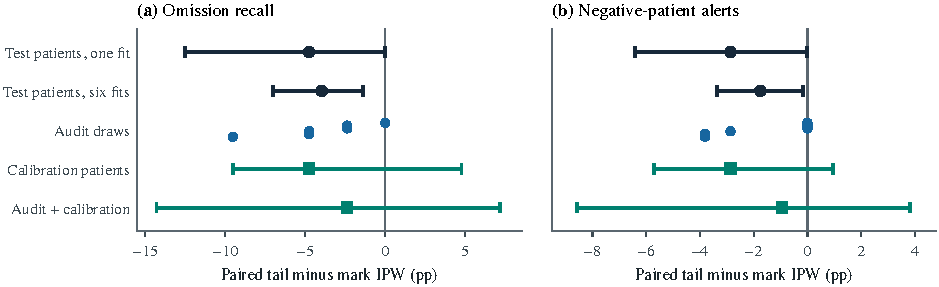
\includegraphics[width=\textwidth]{variability}
\caption{\textbf{Audit, calibration, and test-patient variation answer different questions.}
Dark intervals resample test patients jointly conditional on the fitted heads and cutoffs.
Blue points vary the training audit seed with the original calibration pool fixed.
Green spans summarize the central 95\% of the matched calibration resamples at the anchor and across all fits.
The resampled calibration results use the same test patients.}
\label{fig:variation}
\end{figure*}

\section{Replaying Reference Membership at Fixed Scores}

\paragraph{Two released references.}
The C/D pool contains patients without a concordant contour under the original geometry. The augmented pool also requires no entry in the official LUNA16 annotation file. Candidate matching to official marks for visualization uses the same proposal tolerance, the greater of 3\,mm and half the official diameter. Patient eligibility uses the presence of any official target on that scan, regardless of whether a proposal matches it. Changing membership preserves the original localization targets. This allows a comparison of thresholds without changing the recall denominator. Under both cutoffs the alert denominator in the reference analysis includes only the 90 common-negative test patients.

\begin{table*}[t]
\centering\small
\caption{\textbf{Reference effects by feature family.} Each row summarizes distinct fixed score vectors. Past size band counts rank displacements above the upper end of the central 95\% random-deletion band. More omissions counts heads with strictly more calls under the augmented cutoff.}
\label{tab:families}
\begin{tabular}{lrrrrr}
\toprule
Features & Score vectors & Lower threshold & Past size band & More omissions & Median ranks \\
\midrule
Descriptors & 24 & 24 & 4 & 11 & 3 \\
Multi-view & 2 & 2 & 2 & 2 & 6.5 \\
3D & 257 & 254 & 196 & 238 & 6 \\
\bottomrule
\end{tabular}

\end{table*}

\begin{table*}[t]
\centering\small
\caption{\textbf{Paired-tail differences under each calibration reference.} Six matched fits are averaged within each patient. Both references use the same original targets and 90 common negatives in evaluation. Differences and conditional patient intervals are in percentage points.}
\label{tab:alt}
\begin{tabular}{llrrr}
\toprule
Baseline & Cal. pool & Omit. diff. [95\%] & All diff. [95\%] & Alert diff. [95\%] \\
\midrule
Mark IPW & C/D & -4.0 [-7.0, -1.4] & +3.0 [+1.3, +4.9] & -1.5 [-3.1, +0.0] \\
Mark IPW & + official & +3.6 [-1.4, +9.5] & +6.0 [+3.8, +8.4] & +1.1 [-0.8, +3.4] \\
Mark, same head & C/D & -4.4 [-8.3, -0.8] & -1.3 [-3.0, +0.4] & -2.0 [-4.2, -0.4] \\
Mark, same head & + official & +4.4 [-0.9, +10.0] & +4.8 [+3.0, +6.7] & +0.9 [-0.7, +2.7] \\
First read & C/D & -6.3 [-15.1, +0.0] & -6.2 [-9.3, -3.4] & +0.7 [+0.2, +1.5] \\
First read & + official & -6.0 [-12.2, -1.6] & -3.8 [-6.2, -1.4] & +1.7 [-0.6, +4.3] \\
\bottomrule
\end{tabular}

\end{table*}

\begin{table}[t]
\centering\small
\caption{\textbf{Reader roles at the anchor.} Cells give original omission calls out of 42 and alerts among \RoleTest{} common negatives.}
\label{tab:roles}
\begin{tabular}{lrrrr}
\toprule
Pair & Cal. neg. & First read & Mark IPW & Paired tail \\
\midrule
AB & 66 & 6 / 0 & 3 / 1 & 1 / 0 \\
AC & 72 & 6 / 0 & 3 / 1 & 1 / 0 \\
AD & 63 & 6 / 0 & 3 / 1 & 5 / 1 \\
BC & 68 & 6 / 3 & 4 / 1 & 2 / 0 \\
BD & 65 & 6 / 0 & 3 / 1 & 2 / 0 \\
CD & 67 & 4 / 0 & 3 / 1 & 1 / 0 \\
\bottomrule
\end{tabular}

\end{table}

\paragraph{Fit coverage and the extra architecture.}
We recompute the original cutoffs and all recorded C/D counts at $\alpha=0.10$ before evaluating the augmented membership for every locked observed-arm fit. As a separate architecture check, we use the epoch-16 2.5D checkpoint from the first development screen. Its inputs are twelve planes centered on the candidate, with two physical fields of view. It uses two 24-channel blocks, two 40-channel blocks, and two 64-channel blocks with two intervening pooling operations. Its embedding concatenates center and global means before the 32-channel projection. At export it averages the patch and its separate in-plane flips. We freeze the checkpoint and fit the first-read and full-reference linear heads on the original fitting set at the common ridge. We use the epoch-16 2.5D checkpoint here to test reference sensitivity in a second learned representation. It extends the reference stress test, with the same patient data and proposal source. Identical candidate score vectors are fingerprinted for the descriptive head summary. These fits share the same patient cohort.

\paragraph{Matched random deletion.}
Use one random subset within each of the two original calibration folds, retaining exactly the number that remain under the augmented definition. Repeat 8,192 times with common random draws across the heads. For each deletion take the same 49th order statistic used by the augmented pool. Locate that score in the sorted original pool, with deterministic roster-order tie handling. The random distribution answers how far the cutoff would move if patients were removed uniformly within each fold at the same sample size. The observed displacement uses the same original rank scale. The descriptive tail area in the ledger is the fraction of random displacements at least as large, with a one-draw correction.

\paragraph{Alternative pair memberships.}
Reparse the four LIDC sessions with the original geometry. For each of the six possible unordered pairs, reconstruct pair consensus without scores and verify that C/D reproduces the locked target count on every retained scan. Calibrate on the negatives of each pair and apply the resulting cutoffs to the original target list. The test alert support is the intersection of negatives for the six pairs and the official list, with \RoleTest{} patients. This design isolates sensitivity to reader assignment. Each pair reuses the same unblinded records.

\paragraph{Uncertainty and provenance.}
Compute paired test-patient intervals with 4,000 bootstrap samples after averaging the matched audit fits within each patient. When comparing references, the scores, calibration pools, and cutoffs are held fixed for this bootstrap. The intervals describe variation across test patients under those settings. The blocked random deletion distribution varies only the calibration membership. The follow-up plan was specified after an initial anchor reference check. The prior training and allocation protocol specifies the locked comparison. The output ledgers include the original-fit metrics replay, reference membership, head fingerprints, cutoff order, random-deletion distribution, alert counts, and target calls. The figures are generated from the measured ledgers and staged CT images.

\section{Earlier estimator check}

The historical controlled simulation holds a finite synthetic population and its auxiliary fit fixed and varies the audits and dependence between weak readers. The base-budget augmented prevalence estimate reduced RMSE by about 10--12\% versus the Horvitz--Thompson estimate. The estimand is the proportion of positives among first-reader-unmarked proposals. The image-conditioned bookmark intervention and observed-reader CT endpoints above are localization experiments with different estimands.

\FloatBarrier
\section*{LLM Usage Statement}
OpenAI Codex assisted with experimental design, implementation, analysis, data-derived figures, literature verification and writing.

{\small
\bibliographystyle{ieeenat_fullname}
\bibliography{references}
}
\end{document}
